\input devHead.tex
\SetTheme{AnnArbor} %11
\title{ソフトウェア開発\\第14回目授業}
\author{平野 照比古}
\institute{}
\date{2018/1/18}
\newtheorem{Prob}{解説}
\newcommand{\Elm}[1]{\texttt{<#1>}}
\setbeamercovered{transparent}

\newcommand{\DOMM}{\texttt}
\newcommand{\Event}{\texttt}
\newcommand{\DOMP}{\texttt}
\newcommand{\DOM}{\texttt{DOM}}
\newcommand{\keyitem}{\relax}
\newcommand{\HTML}{HTML文書}
\begin{document}
\frame{\maketitle}
\section{コードの構造}
\subsection{良いコードとは}
 \begin{frame}[containsverbatim]
  \frametitle{良いコードとは}
多くの公開されているコードを眺めているといくつかの共通点が
  見つかる。
\begin{itemize}
 \item プログラムの構造がわかりやすくなるように字下げ(インデント)を付け
			 る。
 \item 変数名や関数名は実体を表すようにする。\\いくつかの単語をつなげて
			 変数名や関数名にすることが多くなる。これらが読みやすいように途中に出てく
			 る単語の先頭は大文字にすることが最近の傾向である(キャメル形式と呼
			 ばれる)。
 \item 不必要に長いプログラム単位を作らない。\\
			 ある程度まとまった作業をする部分は関数にすると見通しの良いプログ
			 ラムとなる。
 \item プログラム自体が説明書になっている。\\
			 コメントを多用して必要な説明をすべて記述する。
\end{itemize}
 \end{frame}
 \begin{frame}[containsverbatim]
  \frametitle{プログラムとデータの分離}
  \begin{itemize}
   \item ある処理をするときの分岐の条件をプログラム内に直接記述すると、分
			 岐の条件が変わったときにはプログラムをコンパイルしなおす必要が生
         ずる。
   \item これを避けるためには外部からデータを読み込んで、それに基づ
			 いた処理を行うようにする。

  \end{itemize}
 \end{frame}
\subsection{プログラムとデータの分離}
 \begin{frame}[containsverbatim]
  \frametitle{成績評価}
  期末試験の結果成績をつける。
  \begin{itemize}
   \item 90点以上ならば\texttt{S}
   \item 80点以上ならば\texttt{A}
   \item 70点以上ならば\texttt{B}
   \item 60点以上ならば\texttt{C}
   \item それ以外は\texttt{E}
  \end{itemize}
 期末試験の点
 を与えて、評価の\texttt{S}などを返す関数\texttt{seiseki}を作成する。
\end{frame}
 \begin{frame}[containsverbatim]
  \frametitle{簡単な方法(JavaScript)}
\begin{Verbatim}
function seiseki(val) {
  if(val >= 90) return "S";
  if(val >= 80) return "A";
  if(val >= 70) return "B";
  if(val >= 60) return "C";
  return "E";
}
\end{Verbatim}
\end{frame}
\begin{frame}[containsverbatim] 
\frametitle{配列の利用(1)}
\begin{Verbatim}
function seiseki(val) {
  var Score = [90,80,70,60,0];
  var Results= ["S","A","B","C","E"];
  var i;
  for(i=0;i<Grade.length;$i++) {
    if(val>=Grade[i]) return Hyouka[i];
  }
  return "Error";
}
\end{Verbatim}
\end{frame}
\begin{frame}[containsverbatim]
 \frametitle{配列の利用(2)}
 配列をまとめる。
\begin{Verbatim}
var Results =[["S",90],["A",80],["B",70],["C",60],["E",0]];
\end{Verbatim}
 連想配列の利用
\begin{Verbatim}
var Results ={S:90,A:80,B:70,C:60,E:0};
function seiseki(val) {
  for(v in Results) {
    if(val >=Results[v]) return v;
  }
}
\end{Verbatim}
JavaScriptでは\texttt{for(.. in ..)}で連想配列の要素をすべて渡ることがで
き、かつわたる順序が定義された順なのでこのコードが可能
\end{frame}
\begin{frame}[containsverbatim]
 \frametitle{JavaScriptにおける注意}
\begin{itemize}
 \item JavaScript内から外部ファイルを自動で読み込むことがで
きない
 \item 変数の形で値を用意
 \item この変数部
分を別のプログラムから作成する方法も可能
\end{itemize}
\end{frame}
\section{コードの管理}
 \begin{frame}[containsverbatim]
  \frametitle{複数でシステム開発をするときの問題点}
\begin{itemize}
 \item 複数の人間で開発している場合、開発者の間で最新のコードの共有
 \item ファイルを間違って削除したり、修正がうまくいかなかったときに過去
       のコードに戻す
 \item 安定しているコードに新規の機能を付け加えてテストをする場合、安定
       したコードに影響を与えないようにする
\end{itemize}
このようなコードの変更履歴の管理するソフトウェアをバージョン管理ソフ
トという。バージョン管理ソフトウェアの対象となるファイルはテキストベース
のものを主としている。
 \end{frame}
\subsection{バージョン管理の概念}
\begin{frame}[containsverbatim]
 \frametitle{バージョン管理ソフトとは}
バージョン管理ソフトは各時点におけるファイルの状態を管理するデータベース
 である。このデータベースは一般にリポジトリと呼ばれる。
\end{frame}
\begin{frame}[containsverbatim]
 \frametitle{バージョン管理ソフトを用いた開発手順}
\begin{itemize}
 \item リポジトリからファイルの最新版を入手
 \item ローカルな環境でファイルを変更。
 \item ファイルをリポジトリに登録
\end{itemize}
\end{frame}
\begin{frame}[containsverbatim]
 \frametitle{バージョン管理ソフトを用いた開発手順の問題点}
\begin{itemize}
 \item 同じファイルを複数の開発者が変更した場合、競合が
発生していないかをチェックする機能
 \item この機能がない場合には
同じファイルの変更は同時に一人しか変更ができないようにファイルをロック
\end{itemize}\end{frame}
\begin{frame}[containsverbatim]
 \frametitle{開発の流れ}
 \begin{itemize}
  \item 開発の流れをブランチと呼ぶ
  \item あるブランチに対して新規の
機能を付け加えたいときなどには元のブランチには手を付けずに別のブランチを
作成して、そこで開発
  \item 機能が安定すれば元のブランチに統合(merge)
 \end{itemize}
\end{frame}
\subsection{バージョン管理ソフトの概要}
\begin{frame}[containsverbatim]
 \frametitle{CVS(Concurrent Versions System)とSubversion}
 \begin{itemize}
  \item 管理するためにサーバーが必要
  \item 開発者はこのサーバーにアクセスしてファ
イルの更新などを行う
 \end{itemize}
\end{frame}
\begin{frame}[containsverbatim]
 \frametitle{gitの場合}
 \begin{itemize}
  \item 各開発者のローカルな環境にサーバー上のリポジトリの複製
を持つ
  \item ネットワーク環境がない状態でもバージョン管理が行える
  \item git ではネットワーク上に GitHub と呼ばれるサーバーを用意しており、ここに
リポジトリを作成することで開発者間のデータの共有が可能
  \item データを公開すれば無料で利用できる
  \item 有料のサービスやサーバー自体を個別に持つサービスも提供
  \item 有名なオープンソースのプロジェクトが GitHub を利用
 \end{itemize}
\end{frame}
\subsection{gitの使い方}
\begin{frame}[containsverbatim]
 \frametitle{git の特徴}
詳しい使い方は \Verb+https://git-scm.com/book/ja/v2/+を参照
\begin{itemize}
 \item 分散型のバージョンシステムなので、ローカルでブランチの作成が可能

       集中型のバージョン管理システムではブランチの作成が一部の人しかで
       きない。
 \item 今までのファイルの変更履歴などが見える。
 \item  GitHub 上ではファイルの更
       新などの通知を受けることができる。
 \item 開発者に対して変更などの要求が可能(pull request)
\end{itemize}
\end{frame}
\begin{frame}[containsverbatim]
 \frametitle{git のインストール}
 \begin{itemize}
  \item git はローカルにリポジトリを持つのでそれを処理する環境をインストー
        ルする
  \item git for windows が良い
  \item 「Git Bash」、「GitCMD」と「Git GUI」の3つがインストールされる。
  \item Unix 風のコマンドプロンプトが起動する Git Bash がおすすめ
 \end{itemize}
\end{frame}
\begin{frame}[containsverbatim]
 \frametitle{初期設定}
 \begin{itemize}
  \item GitHubで使用するリポジトリのユーザ名を登録

        \Verb+git --config --global user.name "Foo"+

ここでは\Verb+Foo+がユーザ名となる。
  \item GitHubからの通知を受けるメールアドレス

        \Verb+git --config --global user.email "Foo@example.com"+
 \end{itemize}
 \end{frame}
\begin{frame}[containsverbatim]
 \frametitle{SSH Keyの登録}
 \begin{itemize}
  \item GitHub との接続には SSH による通信で行う
  \item この通信はは公開鍵暗号方式で行う
  \item キーの生成は次のコマンドで行う
  \item \Verb+ssh-keygen -t rsa -C "Foo@example.com"+

\Verb+-C+のオプションはコメント 
  \item キーを保存するフォルダが聞かれるが、デフォルトでかまわない
  \item passphrase の入力が求められる
  \item 指定したフォルダの\Verb+.ssh+の下に\Verb+id_rsa+(秘密鍵)と
\Verb+id_rsa.pub+(公開鍵)の2つのファイルが作成される。 
 \end{itemize}
\end{frame}
\begin{frame}[containsverbatim]
 \frametitle{GitHub のアカウントの取得}
 \begin{itemize}
  \item ローカルだけで開発をするのであればアカウントは不要
  \item データを交換するのであればアカウントを取ることを勧める
  \item 作成した公開鍵の内容をアカウントで設定する
  \item アカウントを取ったら GitHub 上でテストのプロジェクトを中身が空で作成
 \end{itemize}
\end{frame}
\begin{frame}[containsverbatim]
 \frametitle{リポジトリの作成と運用}
リポジトリの初期のブランチ名は\Verb+master+

 \footnotesize
\begin{tabular}{|c|c|c|}\hline
コマンド&パラメータ&説明\\\hline
\Verb+git init+ & &プロジェクトの初期化\\\hline
\Verb+git add+ & ファイルリスト&プロジェクトへのファイルの登録 \\\hline
\Verb+git commit+& \Verb+-m+ コメント& リポジトリへの変更の登録\\ \hline
\Verb+git remote add+ &短縮名 リポジトリ & リポジトリの短縮名の登録\\
 \hline
\Verb+git push+ &\Verb+-u+ 短縮名 ブランチ名 &ブランチへの変更の登録 \\ \hline
\Verb+git clone+ &リポジトリ名 &リモートのリポジトリのコピーを作成\\ \hline
\Verb+git pull+ &リポジトリ名 ブランチ名 &リモートのリポジトリのコピーを作成\\ \hline
\end{tabular}
\end{frame}
\begin{frame}[containsverbatim]
 \frametitle{新しいプロジェクトの構成}
\begin{enumerate}
 \item \Verb+git init+ で新たにリポジトリを作成、または、
			 \Verb+git clone+でGitHubからリポジトリのコピーを取得する。
 \item ファイルを編集
 \item 編集したファイルを\Verb+git add+ でステージ
 \item \Verb+git commit+ でその時点での変更を登録
 \item \Verb+-m+オプションで簡単なコメントをつけることを忘れないこと。
 \item このオプションをつけないと\Verb+vim+というテキストエディタが立ち
       上がり、コメントの編集を行う
 \item \Verb+git push+ リモート名 ブランチ名 で変更をリモートのリポジト
			 リに反映される。
 \item これが拒否された場合には誰かが\Verb+push+している
			 のでその変更を\Verb+pull+してから調整して再度\Verb+push+する。
\end{enumerate}
\end{frame}
\begin{frame}[containsverbatim]
 \frametitle{ファイルの状態の注意}
\begin{itemize}
 \item リポジトリ内のファイルは追跡されている(tracked)ものと追跡されていない
(untracked)に分けられる。
 \item ファイルの状態として変更されていない
(unmodified)、変更されている(modified)とステージされている(staged)の3つ
の状態がある。
 \item modified から staged にするコマンドが \Verb+git add+ であ
る。このコマンドを新規にリポジトリに追加するという意味にとらえないことが
必要である。
\end{itemize}
\end{frame}
\section{分散処理}
\begin{frame}[containsverbatim]
 \frametitle{分散処理とは}
 \begin{itemize}
  \item あるデータを処理するためにはいくつかのプログラムが必要
  \item そのプログラムの実行単位をプロセスと呼ぶ。
  \item プロセスは他のプロセスと環境が独立しており互いに直接、データの参
        照ができない。
  \item プロセス間でデータを交換するための機能としてプロセス間通信がある。
 \end{itemize}
\end{frame}
\begin{frame}[containsverbatim]
 \frametitle{スレッド}
 \begin{itemize}
  \item 最近のOSではプロセスの中で並行処理が可能となるスレッドが提供され
        ている。
  \item スレッドはプロセスとは異なり、スレッド間でプロセス内のデータを共
        有することが可能
  \item 共有されるデータの書き込みに関しては複数のスレッドから同時に書き込み
        が起きないようにするなどの注意が必要
  \item それができる機能をOSは提供
 \end{itemize}
\end{frame}
\begin{frame}[containsverbatim]
 \frametitle{Web Workers}
 \begin{itemize}
  \item JavaScriptで並行処理を行う機能を提供するものとしてWeb Workerオブジェクト
が提案
 %\footnote{\texttt{https://www.w3.org/TR/workers/}\label{webworkers}}。
  \item Workerオブジェクトは呼び出されるプログラムとは別のメモリー空間で
        実行
  \item 元のプログラムとのデータ交換はメッセージの通知というイベントを通
        じて行う。
  \item Web Workers はプロセス間通信に似た環境を提供している
 \end{itemize}
\end{frame}
\begin{frame}[containsverbatim]
 \frametitle{素数の数を求める}
 $10,000,000$以下の素数を$1,000,000$ずつの区間に分けてその区間
 内にある素数の数をWeb Workers を使用して求めるプログラム

 \hspace*{\fill}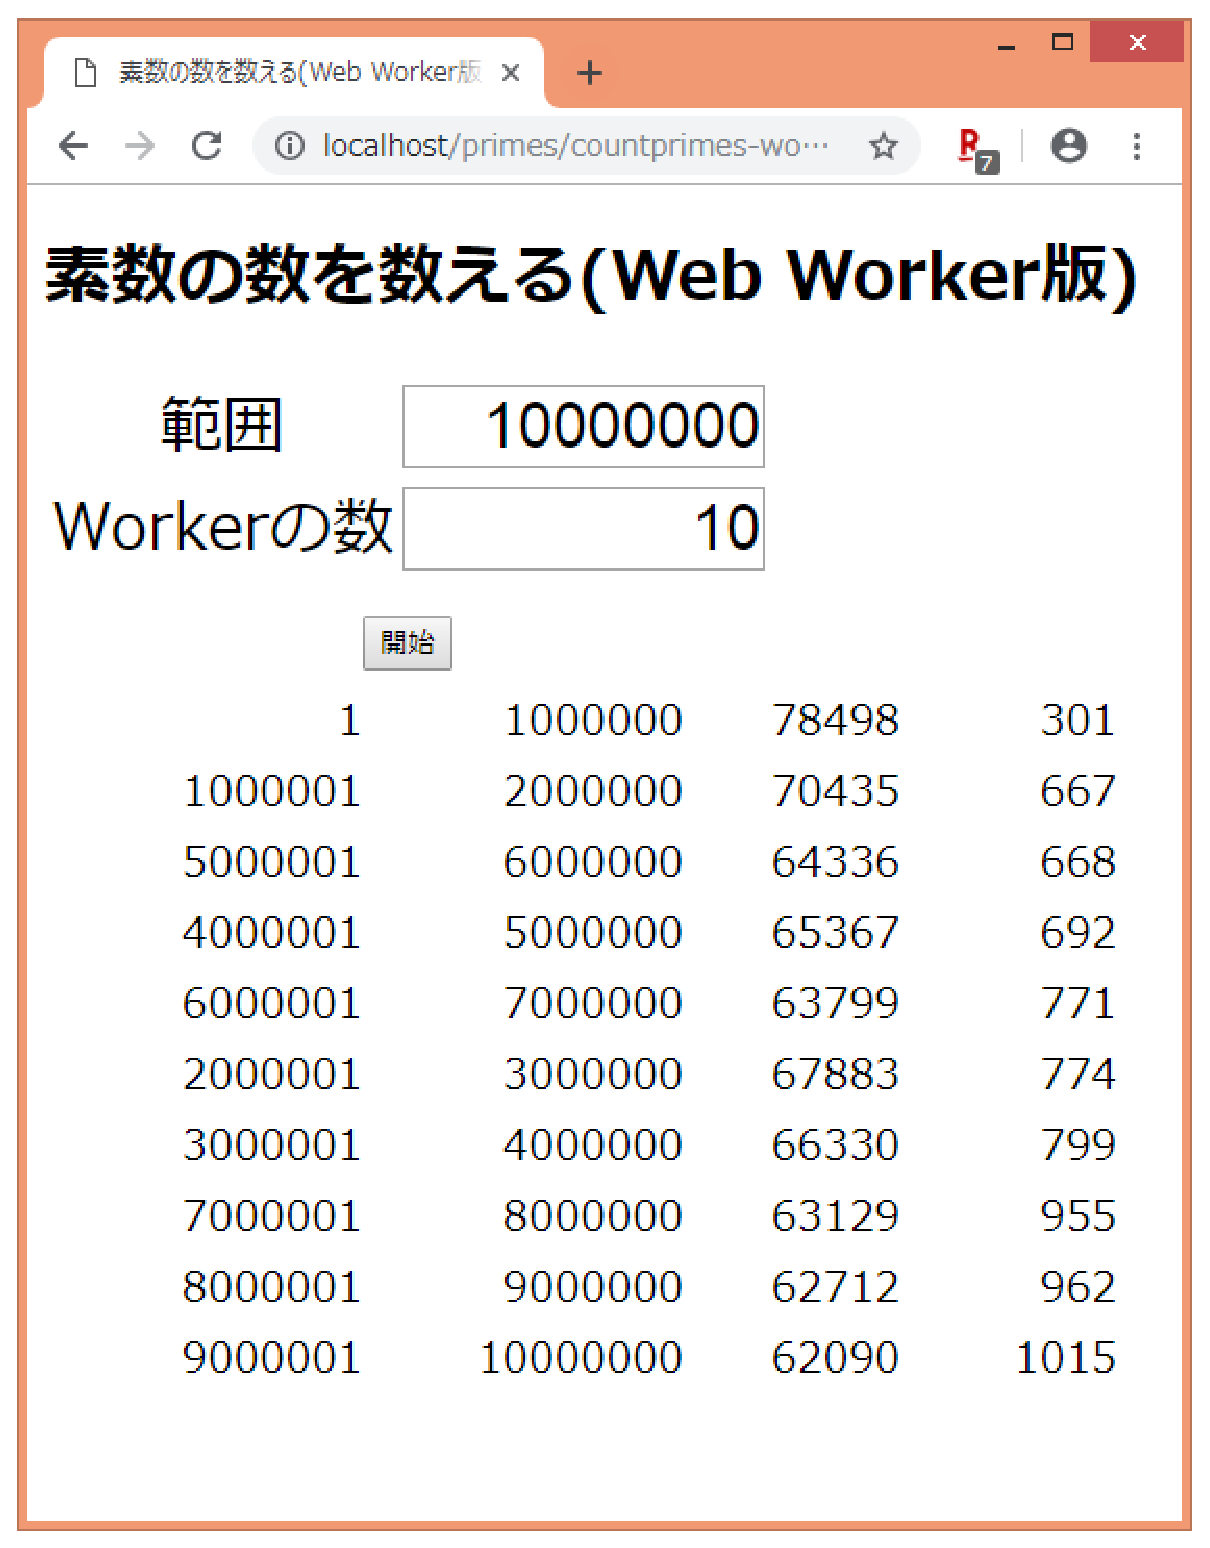
\includegraphics[width=0.3\textwidth]{../primes/countPrimes-workers-res.eps} \hspace*{\fill}
 
項目は左から区間の下限と上限、その区間に含まれる素数の数、開始時間からその区間の実行
 終了までの時間(ミリ秒単位)
\end{frame}
\begin{frame}[containsverbatim]
 \frametitle{素数の数を求める--HTMLファイル}
 \LISTN{../primes/countPrimes-workers.html}{1}{last}{\tiny}
\end{frame}
\begin{frame}[containsverbatim]
 \frametitle{素数の数を求める--HTMLファイル(解説)}
 \begin{itemize}
  \item 5行目で Workerを起動し、その結果をを処理するJavaScriptっ
        ファイルを読み込む。
  \item 6行目でこのページに適用されるスタイルシートの読み込む。
  \item 13行目から16行目で素数の個数を求める範囲を指定するテキストボック
        スを配置
   \item 17行目から20行目で同時に発行するWorkerの個数を指定するテキストボック
        スを配置
  \item 17行目から20行目で計算開始するボタンを配置
 \end{itemize}
\end{frame}
\begin{frame}[containsverbatim]
 \frametitle{素数の数を求める--CSSファイル}
 \LISTN{../primes/primes.css}{1}{last}{\tiny}
\end{frame}
\begin{frame}[containsverbatim]
 \frametitle{素数の数を求める--CSSファイル(解説)}
 \begin{itemize}
  \item 1行目から4行目はテキストボックスに適用される。このページのテキス
        トボックスは数が入力されるので、文字列を右寄せに(2行目)
  \item 5行目から7行目では\texttt{table}要素内の\texttt{td}要素の文字の
        大きさを指定
  \item 8行目から12行目では素数の個数を表示する\texttt{table}要素ないの
        \texttt{td}要素の文字の位置(9行目)、文字の大きさ(10行目)と表示幅
        (11行目)を指定
  \item 13行目から15行目では右2つの\texttt{td}要素の幅を前の2つと異なる
        値に設定(\texttt{100px})
 \end{itemize}
\end{frame}
\begin{frame}[containsverbatim]
 \frametitle{素数の数を求める--JavaSCriptファイル(1)}
 \LISTN{../primes/countPrimes-workers.js}{1}{3}{\tiny}
行目と3行目で\texttt{form}要素と結果を表示するための
 \texttt{table}要素を得ている。
\end{frame}
\begin{frame}[containsverbatim]
 \frametitle{素数の数を求める--JavaSCriptファイル(2)}
  4行目から39行目は「開始」ボタンが押されたときの処理
 \LISTN{../primes/countPrimes-workers.js}{4}{14}{\tiny}
\end{frame}
\begin{frame}[containsverbatim]
 \frametitle{素数の数を求める--JavaSCriptファイル(解説)}
 \begin{itemize}
  \item 5行目ではボタンの操作ができないようにしている。
  \item 6行目から8行目は結果を表示している内容を消去するために、
        表示する要素である\texttt{table}要素を取り除き(6行目)、そ
        の要素だけのコピー(子要素はなし)を作成(7行目)てそれを再び、
        子要素として登録(8行目)している。
  \item 9行目から10行目では素数を求める範囲を最低で$10^{6}$にな
        るようにしている。
  \item 11行目から12行目では区間を分ける数を設定している。
  \item 13行目では個々の処理で求める範囲の幅を求めている。
  \item 14行目ではその時点での時間を求めている。
        \end{itemize}
\end{frame}
\begin{frame}
 \frametitle{素数の数を求める--JavaSCriptファイル(3)}
 \LISTN{../primes/countPrimes-workers.js}{15}{20}{\tiny}
\begin{itemize}
 \item 15行目では発行したWorkersの数を管理する変数を初期化
 \item 17行目から20行目で必要な個数のWeb Workerオブジェクトを作成
 \item Web Workerオブジェクトは\Verb+Worker+コンストラクタで作成
 \item この引数には処理をするJavaScriptファイルを指定
\end{itemize}
\end{frame}
\begin{frame}
\frametitle{素数の数を求める--JavaSCriptファイル(4)}
 \LISTN{../primes/countPrimes-workers.js}{21}{last}{\tiny}
\end{frame}
\begin{frame}[containsverbatim]
 \frametitle{素数の数を求める--JavaSCriptファイル(解説)}
\begin{itemize}
 \item Workerからのメッセージは\Verb+onmessage+イベントを通じて受け取る
 \item この引数は\Verb+message+オブジェクト
 \item \Verb+data+プロパティが送られてきたデータ(26行目)
 \item 送られてきたデータのキーを得て(\texttt{Object.keys})、それぞれを
       \texttt{td}要素内に記述 (29行目)
 \item データが送られてきたので\Verb+worker+の動作を停止し(35行目の
        \Verb+terminate+メソッド)、オブジェクトを消去(36行目)。
\end{itemize}
\end{frame}
\begin{frame}[containsverbatim]
 \frametitle{素数の数を求める--JavaSCriptファイル(Workers)}
 \LISTN{../primes/primes.js}{1}{18}{\tiny}
\end{frame}
 \begin{frame}[containsverbatim]
 \frametitle{素数の数を求める--JavaSCriptファイル(解説)}
 \begin{itemize}
  \item 1行目の\Verb+self+は\Verb+Worker+のもととなるオブジェクトを指す。
        これに\Verb+onmessage+イベントの処理のプログラムを登録
  \item workerが2回目以降呼び出されたかど
				うかを記憶する変数(2行目の変数\texttt{Status})を利用して2回目以
				降の呼び出し時には素数のリストを再度作成しないようにするためにい
				くつかの変数をイベント処理関数の外で定義している(1行目から3行目)。
  \item 最後に\ElmJ{postMessage}メソッドを用いて呼び出し元にデータを送信
        (39行目から40行目)。
  \item 2行目では保存する素数の上限の値を設定している。
        変数\Verb+primes+は小さいほうの素数を配列として格納する。この変
        数は7行目で初期化
  \item 8行目から16行目で残りの素数を求めている。ある数\Verb+i+がその数
        の平方根以下の素数で割り切れないのならば素数と判定できる(11行目)。
 \end{itemize}
 \end{frame}
\begin{frame}[containsverbatim]
 \frametitle{素数の数を求める--JavaSCriptファイル(Workers)}
 \LISTN{../primes/primes.js}{19}{last}{\tiny}
\end{frame}
\begin{frame}[containsverbatim]
 \frametitle{素数の数を求める--JavaSCriptファイル(解説)}
 \begin{itemize}
  \item 19行目以下が与えられた区間における素数の個数を求める部分である。
  \item 開始の値が小さい場合には\Verb+limit+以降から探し、素数の個数を
        \Verb+primes+の長さに初期化する(18行目から21行目)。
  \item 開始の値を奇数に設定し(25行目)、最後の値を求める(27行目)
  \item 29行目から37行目で与えられた区間の奇数が素数であるかの判定を行っ
        ている。この部分は小さい素数を求める部分と同じアルゴリズムである。
  \item 39行目から40行目で結果を送信している。
 \end{itemize}
\end{frame}
\end{document}
